%% Follow comments to support use.

%%%%%%%%%%%%%%%%%%%%%%%%%%%%%%%%%%%%%%%%%%%%%%%%%%%%%%%%%
%% STEP 1: Choose options for MSc / BSc / seminar layout and your bibliographic style
%%%%%%%%%%%%%%%%%%%%%%%%%%%%%%%%%%%%%%%%%%%%%%%%%%%%%%%%%

%%  Language: 
%%      finnish, swedish, or english
%%  Pagination (use twoside by default)  
%%      oneside or twoside,
%%  Study programme / kind of report
%%      csm  = Master's thesis in Computer Science Master's Programme;
%%      tkt = Bachelor's thesis in Computer Science Bachelor's Programme;
%%      seminar = seminar report
%%  For Master's thesis choose your line or track:
%%      (30 cr thesis, 2020 onwards, Master's Programme in Computer Science = csm)
%%      software-track-2020 = Software study track
%%      algorithms-track-2020 = Algorithms study track
%%      networking-track-2020 = Networking study track

\documentclass[finnish,twoside,censored,tkt]{HYthesisML}


% If wanted, open new chapters only at right page.
% By default, "openany".
%\PassOptionsToClass{openright,twoside,a4paper}{report}
\PassOptionsToClass{openany,twoside,a4paper}{report}

\usepackage{csquotes}
%%%%%%%%%%%%%%%%%%%%%%%%%%%%%%%%%%%%%%%%%%%%%%%%%%%%%%%%%
%% REFERENCES
%% Some notes on bibliography usage and options:
%% natbib -> you can use, e.g., \citep{} or \parencite{} for (Einstein, 1905); with APA \cite -> Einstein, 1905 without ()
%% maxcitenames=2 -> only 2 author names in text citations, if more -> et al. is used
%% maxbibnames=99 as no great need to suppress the biliography list in a thesis
%% for more information see biblatex package documentation, e.g., from https://ctan.org/pkg/biblatex 

%% Reference style: select one 
%% for APA = Harvard style = authoryear -> (Einstein, 1905) use:
%\usepackage[style=authoryear,bibstyle=authoryear,backend=biber,natbib=true,maxnames=99,maxcitenames=2,uniquelist=minyear,giveninits=true,uniquename=mininit]{biblatex}
%% for numeric = Vancouver style -> [1] use:
\usepackage[style=numeric,bibstyle=numeric,backend=biber,natbib=true,maxbibnames=99,giveninits=true,uniquename=init]{biblatex}
%% for alpahbetic -> [Ein05] use:
%\usepackage[style=alphabetic,bibstyle=alphabetic,backend=biber,natbib=true,maxbibnames=99,giveninits=true,uniquename=init]{biblatex}
%

\addbibresource{bibliography.bib}
% in case you want the final delimiter between authors & -> (Einstein & Zweistein, 1905) 
% \renewcommand{\finalnamedelim}{ \& }
% List the authors in the Bibilipgraphy as Lastname F, Familyname G,
\DeclareNameAlias{sortname}{family-given}
% remove the punctuation between author names in Bibliography 
%\renewcommand{\revsdnamepunct}{ }


%% Block of definitions for fonts and packages for picture management.
%% In some systems, the figure packages may not be happy together.
%% Choose the ones you need.

%\usepackage[utf8]{inputenc} % For UTF8 support, in some systems. Use UTF8 when saving your file.

\usepackage{lmodern}         % Font package, again in some systems.
\usepackage{textcomp}        % Package for special symbols
\usepackage[pdftex]{color, graphicx} % For pdf output and jpg/png graphics
\usepackage{epsfig}
\usepackage{subfigure}
\usepackage[pdftex, plainpages=false]{hyperref} % For hyperlinks and pdf metadata
\usepackage{fancyhdr}        % For nicer page headers
\usepackage{tikz}            % For making vector graphics (hard to learn but powerful)
%\usepackage{wrapfig}        % For nice text-wrapping figures (use at own discretion)
\usepackage{amsmath, amssymb} % For better math

 \usepackage{listings} % For code formatting
\lstset{literate={ä}{{\"a}}1{ö}{{\"o}}1} % ä and ö support

\singlespacing               %line spacing options; normally use single

\fussy
%\sloppy                      % sloppy and fussy commands can be used to avoid overlong text lines
% if you want to see which lines are too long or have too little stuff, comment out the following lines
% \overfullrule=1mm
% to see more info in the detailed log about under/overfull boxes...
% \showboxbreadth=50 
% \showboxdepth=50



%%%%%%%%%%%%%%%%%%%%%%%%%%%%%%%%%%%%%%%%%%%%%%%%%%%%%%%%%
%% STEP 2:
%%%%%%%%%%%%%%%%%%%%%%%%%%%%%%%%%%%%%%%%%%%%%%%%%%%%%%%%%
%% Set up personal information for the title page and the abstract form.
%% Replace parameters with your information.
\title{Konttien orkestrointi osana DevOps-toimintamallia}

\author{Miko Keskimäki}
\date{\today}

% Set supervisors, use the titles according to the thesis language
% in English Prof. or Dr., or in Finnish toht. or tri or FT, TkT, Ph.D. or in Swedish... 
\supervisors{Lea Kutvonen}

\keywords{DevOps, konttiteknologia, konttien orkestrointi}
\additionalinformation{\translate{\track}}

%% For seminar reports:
%%\additionalinformation{Name of the seminar}

%% Provide classification terms, to appear on the abstract page.
%% Replace the classification terms below with the ones that match your work.
%% ACM Digital library provides a taxonomy and a tool for classification
%% in computer science. Use 1-3 paths, and use right arrows between the
%% about three levels in the path; each path requires a new line.

\classification{\protect{\ \\
\  Software and its engineering $\rightarrow$ Software creation and management $\rightarrow$ Software development process management $\rightarrow$ Software development methods\  \\
\  Computer systems organization  $\rightarrow$ Dependable and fault-tolerant systems and networks  $\rightarrow$ Reliability
}}

%% If you want to quote someone special. You can comment this line out and there will be nothing on the document.
%\quoting{Bachelor's degrees make pretty good placemats if you get them laminated.}{Jeph Jacques}


%% OPTIONAL STEP: Set up properties and metadata for the pdf file that pdfLaTeX makes.
%% Your name, work title, and keywords are recommended.
\hypersetup{
    unicode=true,           % to show non-Latin characters in Acrobat’s bookmarks
    pdftoolbar=true,        % show Acrobat’s toolbar?
    pdfmenubar=true,        % show Acrobat’s menu?
    pdffitwindow=false,     % window fit to page when opened
    pdfstartview={FitH},    % fits the width of the page to the window
    pdftitle={Konttien orkestrointi osana DevOps-toimintamallia},            % title
    pdfauthor={Miko Keskimäki},           % author
    pdfsubject={kanditutkielma},          % subject of the document
    pdfcreator={Miko Keskimäki},          % creator of the document
    pdfproducer={pdfLaTeX}, % producer of the document
    pdfkeywords={DevOps} {konttien orkestrointi}, % list of keywords for
    pdfnewwindow=true,      % links in new window
    colorlinks=true,        % false: boxed links; true: colored links
    linkcolor=black,        % color of internal links
    citecolor=black,        % color of links to bibliography
    filecolor=magenta,      % color of file links
    urlcolor=cyan           % color of external links
}

%%-----------------------------------------------------------------------------------

\begin{document}

% Generate title page.
\maketitle

%%%%%%%%%%%%%%%%%%%%%%%%%%%%%%%%%%%%%%%%%%%%%%%%%%%%%%%%%
%% STEP 3:
%%%%%%%%%%%%%%%%%%%%%%%%%%%%%%%%%%%%%%%%%%%%%%%%%%%%%%%%%
%% Write your abstract in the separate file, to be positioned here.
%% You can make several abstract pages (if you want it in different languages),
%% in which case you should also define the language of the abstract,
%% as below.

\begin{abstract}

DevOps tarkoittaa ohjelmistokehityksen ja IT-toimintojen yhdistämistä.
DevOps-toimintamalli mukainen ohjelmistotuotanto pyrkii automaattiseen laadunvalvontaan ja nopeaan julkaisusykliin.
Toimintamallin mukaista ohjelmistotuotantoa ja sen osana tapahtuvaa jatkuvaa integraatiota ja toimitusta voidaan tukea konttiteknologioiden ja konttien orkestroinnin avulla.
Konttiteknologian avulla samankaltaista vakaan ja toistettavan ympäristön tarjoavaa konttia voidaan käyttää eri vaiheissa toimintamallia.
Konttiorkestrointialustat taas tarjoavat toimintamallia tukevia palveluita testi- ja tuotantoympäristöissä.

Tämän tutkielma tarkastelee DevOps:ia käsitteenä ja konttiteknologian sekä konttien orkestroinnin käyttöä osana DevOps-toimintamallia. Näin tarkoituksena on todeta konttien orkestroinnin ja DevOps-toimintamallin välinen yhteensopivuus.
Konttien orkestroinnin lisäksi käsitellään myös muita mahdollisia ratkaisuja, kuten virtuaalikoneita ja pilvialustoja.
Tutkielmassa esitetään myös käytännön esimerkkin konttiteknologian ja konttien orkestroinnin hyödyntämisestä DevOps-toimintamallin mukaisessa ohjelmistotuotannossa.

\end{abstract}


% Place ToC
%\newpage
\mytableofcontents

\mainmatter

%%%%%%%%%%%%%%%%%%%%%%%%%%%%%%%%%%%%%%%%%%%%%%%%%%%%%%%%%
%% STEP 4: Write the thesis.
%%%%%%%%%%%%%%%%%%%%%%%%%%%%%%%%%%%%%%%%%%%%%%%%%%%%%%%%%
%% Your actual text starts here. You shouldn't mess with the code above the line except
%% to change the parameters. Removing the abstract and ToC commands will mess up stuff.
%%
%% Command \include{file} includes the file of name file.tex.
%% A new page will be created at every \include command, 
%% which makes it appropriate to use it for large entities such as book chapters. Cannot be nested.
%% It is useful for a big project, as changing one of the include targets 
%% won't force the regeneration of the outputs of all the rest.
%% Alternatively, \input is a more lower level macro 
%% which simply inputs the content of the given file like it was copy&pasted there manually.

\chapter{Johdanto\label{intro}}

Konttiteknologiaa käytetään laajalti useilla ohjelmistotuotannon osa-alueilla.
Konttiteknologia mahdollistaa palvelimen suoritusympäristöstä erillisen vakaan ja toistettavan ympäristön \cite{Watada19}.
Konttiorkestraatioalustat hallinnoivat suuria määriä kontteja jaetussa klusterissa.
Orkestraatioalustat, kuten Kubernetes, mahdollistavat muun muassa palveluiden replikoinnin, tehokkaan julkaisuketjun, kontitettujen palveluiden monitoroinnin ja virhetiloista toipumisen \cite{Khan17}.

Konttiteknologiaa ja konttien orkestraatiota käytetään usein osana DevOps-toimintamalliin perustuvaa ohjelmistotuotantoa \cite{Kang16, Narasimhulu23}.
DevOps-toimintamalli pyrkii jatkuvaan integraatioon ja nopeaan julkaisusykliin.
Toimintamalli pohjautuu julkaisun ja laadunvalvonnann osalta tarkasti määriteltyihin automaattisiin prosesseihin \cite{Jabbari16}.

Tämä tutkielma tarkastelee DevOps:ia käsitteenä sekä konttiteknologian ja konttien orkestraation käyttöä osana DevOps-toimintamallia.
Näin tarkoituksena on todeta konttien orkestroinnin ja DevOps-toimintamallin välinen yhteensopivuus.
Yhteensopivuutta arvioidaan määrittelemällä DevOps-toimintamalliin kuuluvia vaiheita ja toimintatapoja sekä arvioimalla konttiteknologian ja konttien orkestroinnin tarjoamia etuja näiden toteuttamiseen.

Konttiteknologian ja konttien orkestroinnin lisäksi käsitellään myös muita mahdollisia ratkaisuja sekä niiden vaikutusta DevOps-toimintamallin mukaiseen ohjelmistotuotantoon.
Lopuksi esitetään käytännön esimerkki tutkielmassa käsiteltyjen teknologioiden ja DevOps-toimintamallin käytöstä.

Luvussa \ref{devops} annetaan määritelmä termille DevOps ja erotellaan siitä tutkielman kannalta merkitykselliset osa-alueet.
Tämän lisäksi kuvataan DevOps-toimintamalliin usein kuuluvia toimintatapoja sekä toimintamallin etuja ja siihen liittyviä haasteita.
Luvussa \ref{orchestration} käsitellään konttiteknologiaa ja konttien orkestrointia sekä niiden sopivuutta osaksi DevOps-toimintamallin mukaista ohjelmistotuotantoa.
Konttien orkestrointia käsitellään erityisesti Kubernetes-konttiorkestrointialustan kautta.

Luvussa \ref{options} käsitellään muita mahdollisia julkaisutapoja ja orkestrointiratkaisuja sekä niiden käyttöä DevOps-toimintamallin kanssa.
Konttiteknologian lisäksi mahdollisina julkaisutapoina käsitellään virtuaalikoneita ja suoraan fyysiselle palvelimelle julkaisemista.
Orkestrointiratkaisuna käsitellään konttien orkestroinnin lisäksi pilvialustojen käyttöä sekä konttien orkestroinnin ja pilvialustan käytön yhdistämistä.
Uutena konttiteknologiaa käyttävänä ratkaisuna mainitaan myös palvelimeton arkkitehtuuri.
Luvussa \ref{example} esitetään käytännön esimerkki DevOps-toimintamallin ja konttien orkestroinnin käytöstä Helsingin yliopiston Norppa-palautejärjestelmän muodossa.
Luvussa kuvataan järjestelmän perustoiminnot, julkaisuputki ja ohjelmistoarkkitehtuuri DevOps-toimintamallin ja konttien orkestroinnin käytön näkökulmasta.

\chapter{DevOps\label{devops}}

DevOps:illa tarkoitetaan ohjelmistokehityksen (engl. \textit{development}) ja IT-toimintojen (engl. \textit{operations}) yhdistämistä.
DevOps:iin liitetään usein jatkuva integraatio ja toimitus sekä automaatio ja laadunvalvonta \cite{Jabbari16, Leite19}.
DevOps:ia käsitteenä voidaan tarkastella ajattelutapana tai käytännön ohjelmistotuotannon toimintamallina.

DevOps ajattelutapana pyrkii ohjelmistokehityksen ja IT-toimintojen jaon välttämiseen ja yhteistoiminnan mahdollistavan kulttuurin rakentamiseen \cite{Klein21}.
DevOps toimintamallina taas keskittyy käytännön toimiin ja teknologioihin, jotka mahdollistavat DevOps-ajattelutavan mukaisen ohjelmistotuotannon.
Tässä tutkielmassa keskitytään aiheen käsittelyyn käytännön toimintamallin kautta.

\section{DevOps-toimintamalli}

DevOps-toimintamalli painottaa jatkuvaa integraatiota ja toimitusta sekä laadunvalvontaa käyttäen standardisoituja automaattisia menetelmiä \cite{Leite19}.
Kuva~\ref{fig:devops} visualisoi DevOps-toimintamallin eri vaiheita.
Kehitys- ja operaatiovaiheet tapahtuvat limittäin ja koko prosessi voidaan suorittaa useita kertoja päivässä automatisoidun julkaisuputken avulla.

\begin{figure}[ht]
\begin{center}
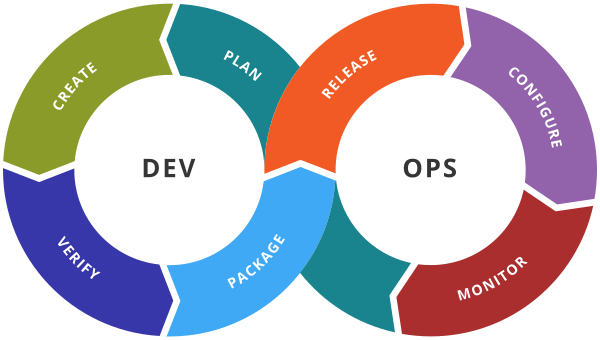
\includegraphics[width=0.6\textwidth]{figures/devops_toolchain.png}
\caption{DevOps-toimintamallin vaiheet.\cite{Wikimedia23}\label{fig:devops}}
\end{center}
\end{figure}

DevOps-toimintamallin vaiheet ja niistä käytetyt termit vaihtelevat lähteestä riippuen, mutta tämän tutkielman osalta käytetään seuraavia vaiheita \cite{Alnafessah21}:

\begin{itemize}
\item Määrittely (engl. \textit{plan}): Ohjelmistotuotannon tavoitteiden määrittely sekä päivitysten ja julkaisuiden alustava suunnittelu.
\item Kehitys (engl. \textit{create, develop}): Määrittelyn mukainen ohjelmisto- ja infrastruktuurikoodin kehitys nopealla versiohallintaan viennillä.
\item Varmennus (engl. \textit{verify, test}): Jatkuva koodin automaattinen testaus ja koodin manuaalinen arviointi tarvittaessa.
\item Julkaisu (engl. \textit{release, deploy}): Uuden ohjelmakoodin julkaisu tuotantoympäristöön ja tuotantoalustan konfiguraatio.
\item Operointi (engl. \textit{operate, configure}): Julkaisun jälkeinen palvelun hallinnointi, resurssien hallinta ja palvelun skaalautuminen.
\item Monitorointi (engl. \textit{monitor}): Palvelun suorituskyvyn ja lokien seuranta, ongelmatilanteisiin reagointi.
\end{itemize}

\section{Jatkuva integraatio ja toimitus}

Jatkuva integraatio ja toimitus (engl. \textit{continuous integration and continuous deployment, CI/CD}) on keskeinen osa DevOps-toimintamallia \cite{Jabbari16, Leite19}. Jatkossa tutkielmassa käsitteisiin viitataan vakiintuneilla lyhenteillä CI ja CD.

CI viittaa koodimuutosten vientiin versionhallintaan nopealla tahdilla ja muutosten automaattiseen testaukseen sen yhteydessä.
CD taas tarkoittaa CI:n seurauksena validoidun koodin automaattista julkaisua tuotantoympäristöön tai sitä muistuttavaan testiympäristöön \cite{Shahin17}.
CI/CD mahdollistaa näin tehokkaan laadunvalvonnan ja ohjelmiston nopean julkaisusyklin.

\begin{figure}[ht]
\begin{center}
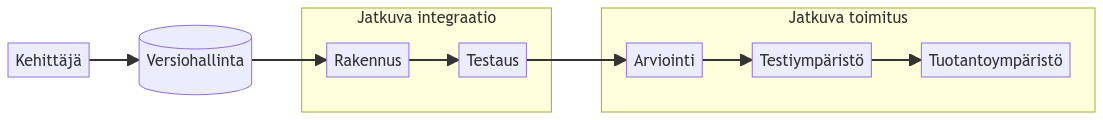
\includegraphics[width=0.8\textwidth]{figures/cicd-pipeline.png}
\caption{Jatkuvan integraation ja toimituksen vaiheet.\label{fig:cicd}}
\end{center}
\end{figure}

Kuva \ref{fig:cicd} esittää esimerkin mahdollisesta CI/CD-putkesta. CI/CD käynnistyy kehittäjän puskiessa uuden koodimuutoksen versiohallintaan.
CI:n aikana uusi version sovelluksesta rakennetaan päivitetystä koodista ja uudelle versiolle suoritetaan automaattiset testit.
Automaattiset testit läpäissyt koodi voidaan tarvittaessa katselmoida ja sovelluksen uusi versio julkaistaan vaiheittain testi- ja tuotantoympäristöihin osana CD:tä.

\section{Haasteet}

DevOps-toimintamalliin perustuva ohjelmistotuotanto luo uusia haasteita.
CI/CD ja toimintamallin vaiheiden seuraaminen nopealla syklillä vaatii automaatiota ja vaiheiden helppoa toistettavuutta \cite{Jabbari16, Leite19}.
Ohjelmistokehittäjien perehdyttäminen DevOps:in mukaisiin toimintatapoihin ja teknologiohiin on yksi haasteista.
Myös DevOps-toimintamallin käyttöönotto sekä toimintamallin seurannan laadun arvioiminen on haastavaa \cite{Leite19}.
Haasteissa painottuvat erityisesti inhimilliset tekijät kuten kommunikaatiohaasteet ja muutosvastarinta \cite{Kalliosaari16}.
Teknisen puolen haasteita ovat taas ohjelmistoinfrastruktuurin hallinta, kuten monimutkaiset kehitys- ja tuotantoympäristöt \cite{Khan22, Kalliosaari16}.

DevOps-toimintamallin käyttöönoton yhteydessä on arvioitava erilaisten teknologioiden soveltuvuuttaa osaksi mallin mukaista ohjelmistotuotantoa.
Sopivilla teknologiavalinnoilla voidaan vähentää ohjelmistoinfrastruktuurin monimutkaisuutta.
Yksi näistä teknologiavalinnoista on julkaisutavan valinta.
Automaation ja toistettavuuden kannalta ratkaisuksi sopisi esimerkiksi virtuaalikoneet tai konttiteknologia \cite{Dua14}.
Konttiteknologiaa ja konttien orkestrointia voidaan käyttää onnistuneesti osana DevOps-toimintamallia \cite{Kang16, Narasimhulu23}.
Seuraavaksi käsitellään näitä aiheita ja arvioidaan niiden yhteensopivuuttaa DevOps-toimintamallin kanssa.

\chapter{Konttien orkestrointi\label{orchestration}}

Konttiteknologiaa ja konttien orkestrointia käytetään monilla ohjelmistotuotannon osa-alueilla.
Konttiteknologia mahdollistaa fyysisen palvelimen tai ohjelmistökehittäjän tietokoneen suoritusympäristöstä eroavan vakaan ja toistettavan ympäristön \cite{Watada19}.
Konttiteknologian kasvava käyttö on luonut tarpeen hallinnoida suuria määriä kontteja samanaikaisesti.
Tähän tarpeeseen pyrkivät vastaamaan erilaiset konttiorkestraatioalustat.

Konttiorkestraatioalustat hallinnoivat suuria määriä kontteja jaetussa klusterissa.
Orkestraatioalustat, kuten Kubernetes, mahdollistavat muun muassa palveluiden replikoinnin, tehokkaan julkaisuketjun, kontitettujen palveluiden monitoroinnin ja virhetiloista toipumisen \cite{Khan17}.

\section{Kontti\label{container}}

% Maybe add something about container runtimes here?

Kontti on karsittu ympäristö, joka koostuu palvelusta ja sen tarvitsemista riippuvuuksista.
Kontti tarjoaa vakaan ja suljetun ympäristön palvelun suorittamiselle \cite{Watada19}.
Kontti on riippumaton fyysisestä palvelimesta ja sen ulkopuolisestä ympäristöstä, joka mahdollistaa saman kontin toistamisen muilla palvelimilla ja alustoilla \cite{Saha18}.

Virtuaalikonejulkaisuista poiketen useampi kontti voi jakaa resursseja ja näin ollen esimerkiksi käyttöjärjestelmän ydintä ei tarvitse säilöä erikseen jokaiseen konttiin.
Tämän seurauksena kontit ovat kokonsa ja käynnistysnopeutensa suhteen virtuaalikoneita tehokkaampi ratkaisu \cite{Dua14}.

% Kuva~\ref{fig:container} esittää resurssien jaon eri julkaisuratkaisuilla.
% Konttijulkaisussa useampi erillisissä konteissa suoritettava sovellus käyttää samaa käyttöjärjestelmän ydintä ja konttien suoritusympäristöä.
% Virtuaalikoneiden ja perinteisten 

Yleisesti käytettyjä konttiteknologiapalveluita ovat Docker ja Podman \cite{Abraham20, Bernstein14}.
Docker on suosittu ratkaisu, mutta vaatii toimiakseen aina käynnissä olevan palveluprosessin ja root-oikeudet palvelua suorittavaan käyttöjärjestelmään \cite{Abraham20}.
Nämä tekniset ongelmat ratkaisee esimerkiksi Podman, joka toimii ilman erillistä palveluprosessia ja root-oikeuksia \cite{Gantikow20}.
Konttiteknologiapalveluiden käyttämiä konttien suoritysympäristöjä (\textit{container runtime}) ovat muun muassa containerd ja CRI-O.
Konttien suoristusympäristöjen vaikutus palvelun suorituskykyyn suoraan palvelimelle julkaisemiseen verrrattuna on hyvin vähäinen \cite{torrez19, espe20}.

% \begin{figure}[ht]
% \begin{center}
% 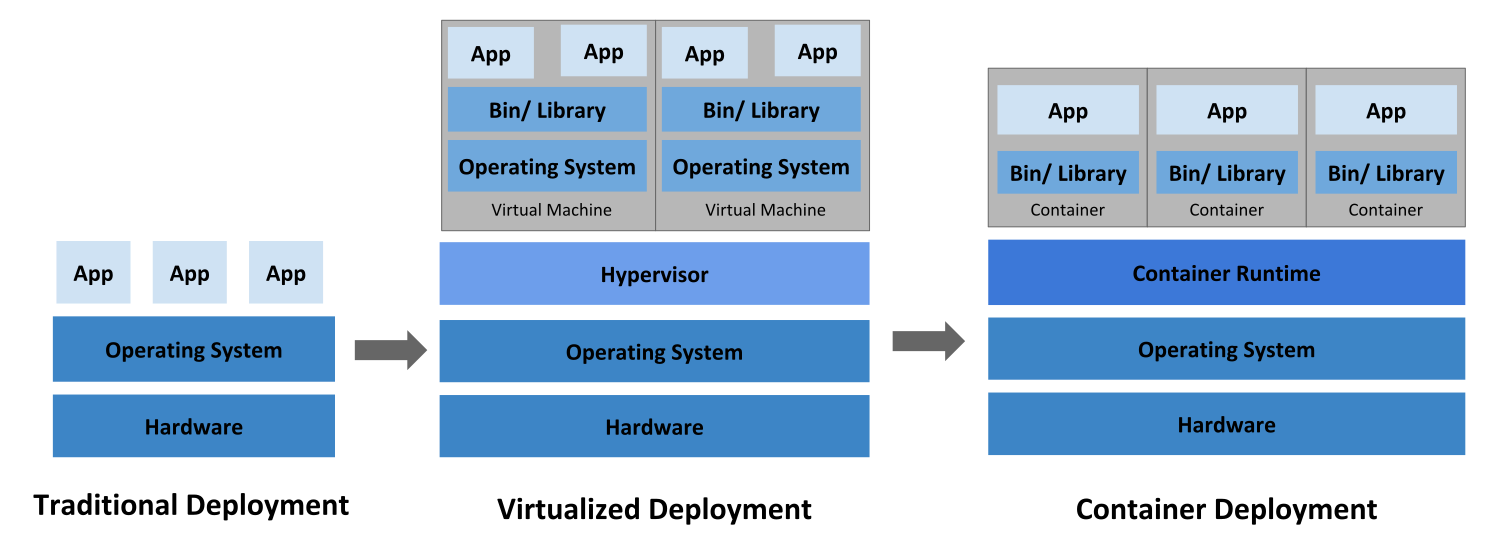
\includegraphics[width=0.9\textwidth]{figures/container_evolution.png}
% \caption{Sovelluksen omat ja jaetut resurssit eri julkaisutavoilla \cite{Kubernetes23}\label{fig:container}.}
% \end{center}
% \end{figure}

\section{Konttiorkestraatioalustat\label{platforms}}

Erityisesti mikropalvelupohjaiset järjestelmät saattavat koostua useista sadoista konteista.
Myös saman palvelun replikaatio ja alueellinen hajauttaminen luovat tarpeen hallinnoida suuria määriä kontteja \cite{Khan17}.
Konttiorkestraatioalustat ovat järjestelmiä, joiden tehtävä on mahdollistaa suurien konttimäärien hallinnointi.
Konttiorkestraatioalustat hallinnoivat konttien resurssien käyttöä, mahdollistavat konttien monitoroinnin ja huolehtivat konttien virhetilanteista toipumisesta \cite{Zhou21}.

Kubernetes on laajalti käytetty konttiorkestraatioratkaisu.
Se on nykyisistä ratkaisuista suorituskyvyltään tehokkain ja myös toiminnallisuuksiltaan kattavin \cite{Jawarneh19}.
Muita ratkaisuja ovat muun muassa Docker Swarm ja Amazon Elastic Container Service \cite{Khan17}.
Tässä tutkielmassa konttien orkestrointia käsitellään pääasiassa Kuberneteksen kautta.

Kubernetes on alkujaan Googlen kehittämä ja nykyään \textit{Linux Foundation}:in osana toimivan \textit{Cloud Native Foundation}:in hallinnoima avoimen lähdekoodin projekti \cite{Burns22}.
Kubernetes hallinnoi podeiksi kutsuttuja yhdestä tai useammasta kontista koostuvia kokonaisuuksia.
Kubernetes-klusteri muodostuu useista fyysisistä palvelimista tai virtuaalikoneista, joita kutsutaan solmuiksi (\textit{node}) \cite{Medel18}.
Kubernetes mahdollistaa muun muassa seuraavat asiat \cite{Zhou21}:

\begin{itemize}
\item Resurssien käyttörajojen hallinta (\textit{resource limit control}): Muisti- ja suoritinresurssien minimi- ja maksimimäärän asettamisen konttikohtaisesti.
\item Vuoronvalvonta (\textit{scheduling}): Konttien automaattinen ja optimoitu sijoitus eri solmujen välillä.
\item Kuormituksen tasaaminen (\textit{load balancing}): Kuormituksen jakaminen useiden saman palvelun konttien välillä. 
\item Terveystarkastus (\textit{health check}): Konttien toimivuuden tarkastus ja viallisiin kontteihin reagointi.
\item Vikasietoisuus (\textit{fault tolerance}): Automaattinen uusien konttien luonti ja viallisten tuhoaminen virhetilanteissa.
\item Automaattinen skaalautuminen (\textit{auto-scaling}): Konttien lisääminen tai poistaminen automaattisesti kuormituksen mukaan.
\end{itemize}

Kuva \ref{fig:kubernetes} esittää Kuberneteksen eri komponentit. Kubernetes-klusteri koostuu useasta podeja suorittavista nodeista.
Koko klusteria hallinnoi \textit{Control Plane}, joka sisältää klusterin hallinnointiin käytetyn REST-rajapinnan, podien jakautumisesta nodejen välillä huolehtivan vuorontajan sekä pysyväistallennetun avainarvosäilön.
Näiden lisäksi \textit{Control Plane} sisältää useita \textit{Controller manager}-prosesseja, jotka hallinnoivat eri resursseja.
Erityisesti \textit{Cloud controller manager} on komponentti, joka mahdollistaa Kubernetes-klusterin yhdistämisen eri pilvialustojen rajapintojen kanssa \cite{components23}.

\begin{figure}[ht]
\begin{center}
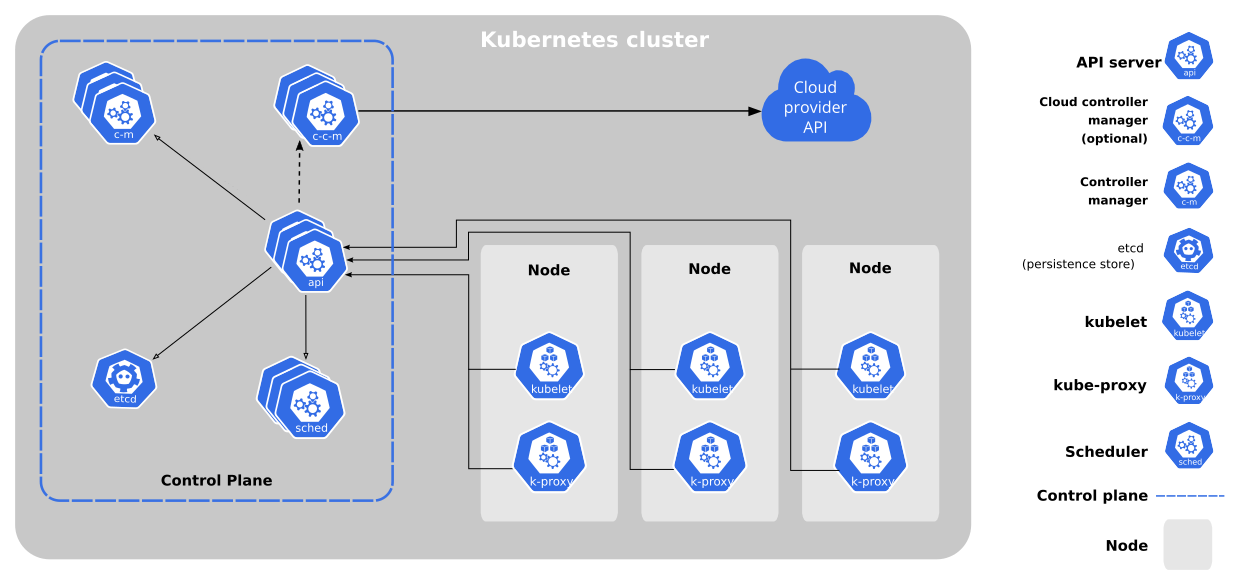
\includegraphics[width=1\textwidth]{figures/kubernetes_components.png}
\caption{Kuberneteksen komponentit \cite{components23}\label{fig:kubernetes}.}
\end{center}
\end{figure}

\section{Konttien orkestrointi DevOps-toimintamallissa\label{orchestration:devops}}

Konttiteknologiaa ja konttien orkestrointia käytetään usein osana DevOps-toimintamalliin perustuvaa ohjelmistotuotantoa \cite{Kang16, Narasimhulu23}.
Konttiteknologia avulla kontitettua palvelua voi siirtää eri ympäristöjen välillä.
Konttiteknologia mahdollistaa myös koko palvelun ympäristön konfiguroinnin ja näin ennustettavamman toiminnan ja helpomman vianmäärityksen \cite{Narasimhulu23}.

Kontin siirrettävyys mahdollistaa tehokkaan varmennus- sekä julkaisuvaiheen DevOps-toimintamallissa, koska samaa konttia voidaan ensin käyttää testauksessa ja sen jälkeen siirtä se esimerkiksi julkaisualustana toimivalle konttiorkestraatioalustalle.
Kontin ympäristön konfiguroitavuus taas auttaa operointi- ja monitorointivaiheissa.
Kontin erikseen määritettävästä ympäristöstä voi olla hyötyä myös kehitysvaiheessa, koska se mahdollistaa useille kehittäjille samanlaisen tuotantoympäristöä muistuttavan kehitysympäristön.

Luvussa \ref{platforms} käsitellyt Kuberneteksen tarjoamat konttien orkestrointipalvelut tukevat myös hyvin DevOps-toimintamallia.
Resurssien käytön hallinta, aikataulutus, kuormituksen tasapainottaminen ja automaattinen skaalautuminen tukevat kaikki hyvin operointivaihetta.
Terveystarkastus ja vikasietoisuus taas tukevat monitorointia.
Konttiorkestraatioalustan käyttö myös itsessään mahdollistaa konttiteknologian käytön palvelun julkaisuratkaisuna, joka tekee saman kontin käytöstä testauksessa ja tuotantokäytössä mahdollista.

Konttiteknologian ja konttien orkestroinnin käytöstä osana DevOps-toimintamallia on löytynyt paljon etuja.
Seuraavaksi tarkoituksena on tarkastella muita julkaisutapoja ja niiden soveltuvuutta DevOps-toimintamallin mukaiseen ohjelmistotuotantoon.
Näitä julkaisutapoja verrataan myös konttiteknologian ja konttien orkestraation käyttöön.

% Decent stuff, but this can be made more explicit, less listlike, see email

\chapter{Muut vaihtoehdot\label{options}}

Konttiteknologian ja konttien orkestraation lisäksi käytössä on muita julkaisutapoja. Konttiteknologian sijaan suoritusympäristön virtualisaatio voidaan toteuttaa virtuaalikoneiden avulla tai palvelua voidaan suorittaa suoraan fyysisellä palvelimella \cite{Watada19}.
Sekä konttien, että virtuaalikoneiden hallinnointiin voidaan käyttää konttiorkestraatioalustan sijaan erilaisia pilvialustoja \cite{Bousselmi14}.
Konttiteknologioiden käytön yleistyminen on myös johtanut uusiin niin sanottuihin Serverless-ratkaisuihin \cite{Baldini17}.

\section{Virtuaalikoneet}

Virtualisaatiolla tarkoitetaan fyysisen laitteen tai resurssin toteuttamista virtuaalisessa muodossa.
Kokonaista virtualisoitua käyttöjärjestelmää kutsutaan virtuaalikoneeksi.
Virtuaalikoneiden avulla yksittäisen fyysisen palvelimen resurssit voidaan jakaa useamman virtuaalisen käyttöjärjestelmän välillä \cite{Smith05}.
Virtuaalikoneiden suoritus tapahtuu virtualisointiympäristössä (engl. hypervisor, virtual machine monitor), joka huolehtii fyysisen palvelimen resurssien abstrahoinnista ja virtuaalikoneiden hallinnoinnista \cite{desai13}.

Virtuaalikoneet mahdollistavat konttien tapaan palvelimesta erillisen toistettavan ympäristön.
Kuvassa \ref{fig:container} esitetään virtuaalikonejulkaisun rakenne.
Luvussa \ref{container} todettiin, että kontti on kokonsa ja käynnistysnopeutensa suhteen virtuaalikoneita tehokkaampi ratkaisu.
Virtuaalikoneiden rakenteelliset erot kontteihin nähden mahdollistavat kuitenkin paremman tietoturvan \cite{Sultan19}.

% What are VMs?
% Benefits, downsides, security
% No orchestration

\section{Fyysiset palvelimet}

% bare metal
% downsides, simplicity and security benefits
% performance?

\section{Pilvialustat}

% Cloud services etc.
% Can orchestrate VMs, containers, bare metal

\section{Serverless}
% Own Section?
% Serverless, new thing, acually containerized?

\chapter{Käytännön esimerkki: Norppa\label{example}}

Helsingin yliopiston tietojenkäsittelytieteen osaston sovelluskehitysakatemian (\textit{Toska}) \cite{Tenhunen23} kehittämä kurssipalautejärjestelmä Norppa on tutkielmassa esitetyn DevOps-toimintamallin mukaisessa aktiivisessa kehityksessä.

\textit{jatkuu}

\begin{figure}[ht]
\begin{center}
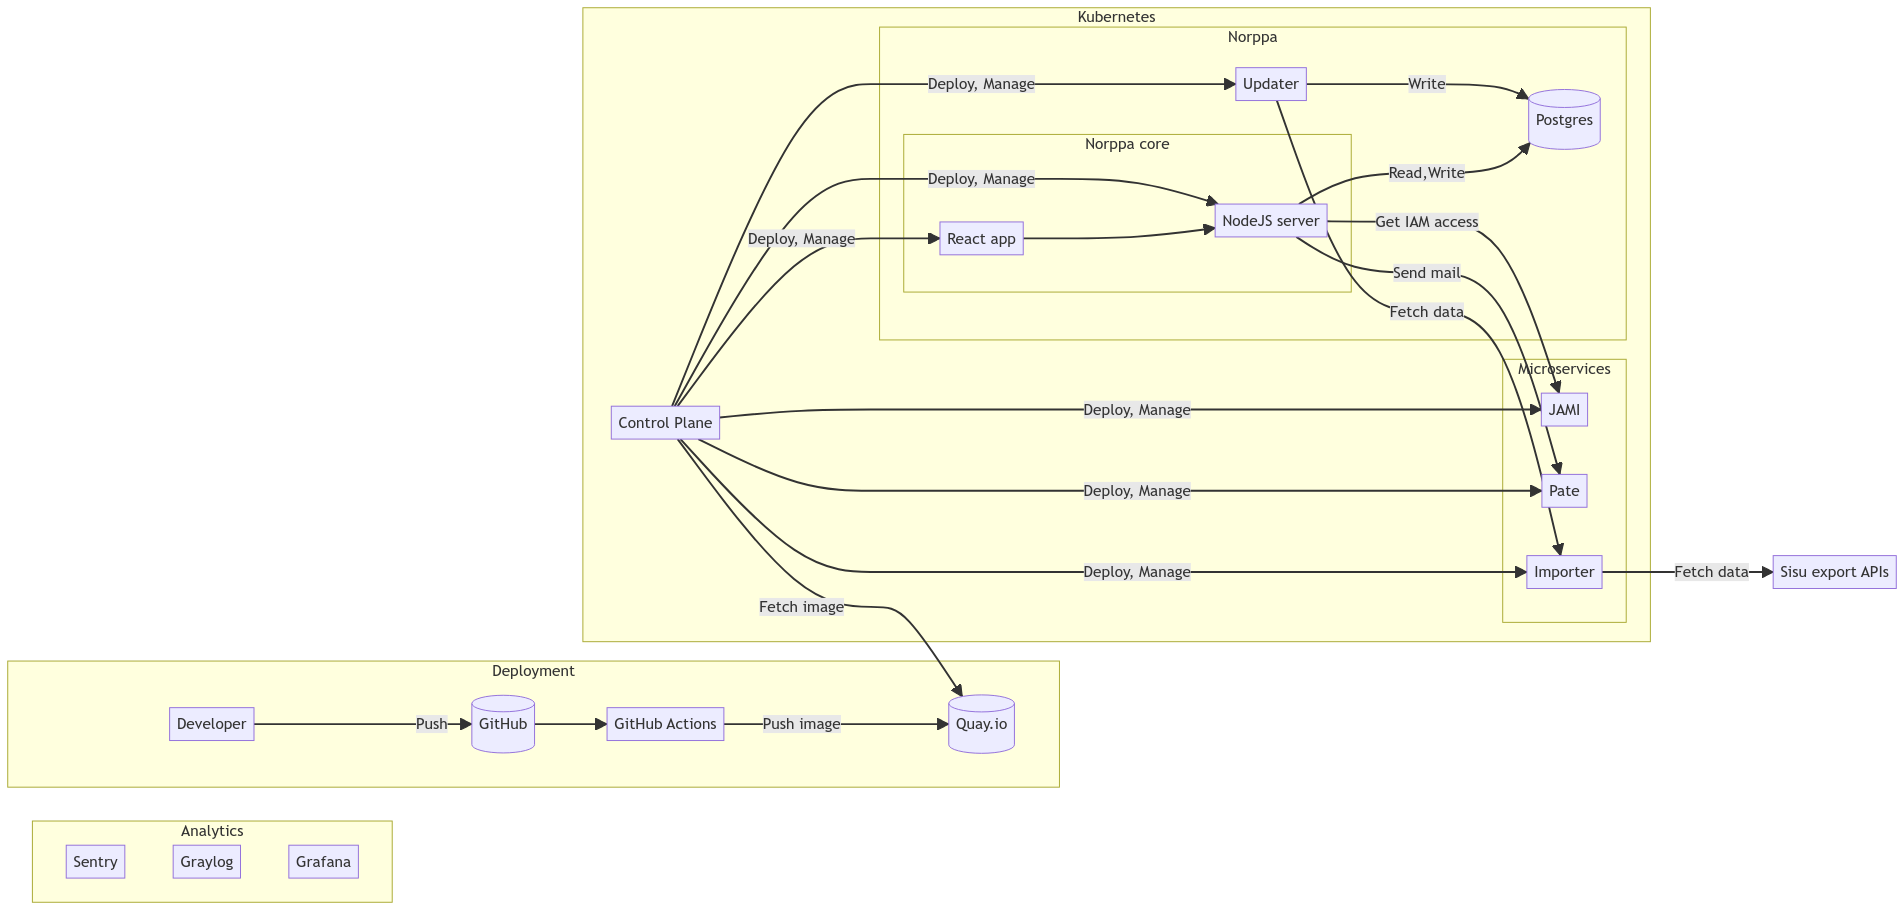
\includegraphics[width=1\textwidth]{figures/norppa_diagram.png}
\caption{Norppa-palautejärjestelmän laajennettu julkaisu- ja arkkitehtuuridiagrammi \cite{Norppa23}\label{fig:norppa}.}
\end{center}
\end{figure}

\chapter{Yhteenveto\label{summary}}

DevOps-toimintamalli perustuu jatkuvaan integraatioon ja toimitukseen sekä toimintamallin vaiheiden mukaiseen ohjelmistotuotantoon.
Jatkuvan integraation ja toimituksen osana koodimuutokset testataan ja viedään testi- ja tuotantoympäristöön nopealla julkaisusyklillä.
Näin uudet koodimuutokset saadaan nopeasti käyttöön ja mahdolliset ongelmatilanteet huomataan nopeasti.

Konttiteknologia ja konttien orkestrointi tukevat DevOps-toimintamallin mukaista ohjelmistotuotantoa.
Konttiteknologian avulla samankaltaista konttia voidaan käyttää ensin testauksessa osana jatkuvaa integraatiota ja myöhemmin tuotantokäytössä konttiorkestrointialustalla.
Konttien orkestrointi mahdollistaa muun muassa resurssien käytön hallinnan, konttien monitoroinnin ja virhetilanteista toipumisen.
Näin konttiorkestrointialustat tukevat DevOps-toimintamallin eri vaiheita.

Virtuaalikoneet mahdollistavat konttiteknologian tapaan vakaan ja toistettavan ympäristön.
Kontteja hitaamman käynnistysnopeuden ja suuremman kokonsa vuoksi ne eivät kuitenkaan sovellu yhtä hyvin orkestrointialustojen käyttöön.
Virtuaalikoneet tarjoavat kuitenkin kontteja paremman eristyneisyyden ja tietoturvan.
Pilvialustat tarjoavat monia DevOps-toimintamallia tukevia palveluita, jotka täydentävät tai osaltaan vähentävät tarvetta konttien orkestroinnille.

Norppa-palautejärjestelmän kehitys on käytännön toteutus DevOps-toimintamallin mukaisesta ohjelmistotuotannosta ja konttien orkestroinnin käytöstä.
DevOps-toimintamallin mukainen ohjelmistotuotanto mahdollistaa esitetyn nopean julkaisuputken ja laadunvalvonnan.
Konttiteknologian ja konttien orkestroinnin mahdollistama ohjelmistoarkkitehtuuri tukee saman palvelun käyttöä ja jatkokehitystä Helsingin ja Tampereen yliopistojen välillä.
Norppa-palautejärjestelmän siirto virtuaalikonepohjaisesta ratkaisusta OpenShift-konttiorkestrointialustalle vähensi ylläpitotaakkaa ja paransi palvelun vakautta ja käytettävyysaikaa.


%%%%%%%%%%%%%%%%%%%%%%%%%%%%%%%%%%%%%%%%%%%%%%%%%%%%%%%%%
%\cleardoublepage                          %fixes the position of bibliography in bookmarks
%\phantomsection
\addcontentsline{toc}{chapter}{\bibname}  % This lines adds the bibliography to the ToC
\printbibliography

%%%%%%%%%%%%%%%%%%%%%%%%%%%%%%%%%%%%%%%%%%%%%%%%%%%%%%%%%
\backmatter
\begin{appendices}

%\appendix{Diagrammien lähdekoodi\label{appendix:diagram}}

\begin{lstlisting}[title=Kuva \ref{fig:cicd}, captionpos=b]
graph LR
    developer[Kehittäjä] --> version[(Versiohallinta)]
    version --> build
    test --> review

    subgraph "Jatkuva integraatio"
        build[Rakennus] --> test[Testaus]
    end

    subgraph "Jatkuva toimitus"
        review[Arviointi] --> staging[Testiympäristö]
        staging --> production[Tuotantoympäristö]
    end
\end{lstlisting}

\begin{lstlisting}[title=Kuva \ref{fig:norppa}, captionpos=b]
graph TB
    sisu[Sisu export APIs]
    importer -->|Fetch data| sisu

    server -->|Get IAM access| jami
    server -->|Send mail| pate
    updater -->|Fetch data| importer

    updater -->|Write| pg
    server -->|Read,Write| pg

    subgraph Deployment
        Developer[Developer] -->|Push| gh
        gh[(GitHub)] --> gha
        gha[GitHub Actions] -->|Push image| quay
        quay[(Quay.io)]
    end

    subgraph Analytics
        sentry[Sentry]
        graylog[Graylog]
        grafana[Grafana]
    end

    subgraph Kubernetes
        control[Control Plane] -->|Fetch image| quay

        control[Control Plane] -->|Deploy, Manage| client
        control[Control Plane] -->|Deploy, Manage| server
        control[Control Plane] -->|Deploy, Manage| updater

        control[Control Plane] -->|Deploy, Manage| jami
        control[Control Plane] -->|Deploy, Manage| pate
        control[Control Plane] -->|Deploy, Manage| importer

        subgraph Norppa

            subgraph Norppa core
                client[React app] --> server[NodeJS server]
            end

            updater[Updater]
            pg[(Postgres)]
        end

        subgraph Microservices
            jami[JAMI]
            pate[Pate]
            importer[Importer]
        end
    end
\end{lstlisting}

\appendix{Tekoälyn käyttö\label{appendix:ai}}

Tutkielman suunnitteluvaiheessa käytettiin GPT-4-kielimallia OpenAI:n rajapinnan kautta.
Kielimallia käytettiin mahdollisten aiheiden generointiin ja aihealueen yleiseen tutkimiseen.
Kielimallia ei ole käytetty tutkielman kirjoituksen aloittamisen jälkeen ja mitään osaa tutkielmasta ei ole tuotettu kielimallin avulla.

DeepL-konekäännöspalvelua on käytetty suomenkielisten vastineiden löytämiseksi joillekin englanninkielisille termeille.
Tämän lisäksi palvelua on käytetty synonyymien etsimiseen.

Lähteiden hakuun, analysointiin tai tiivistämiseen ei ole käytetty tekoälypalveluita.


\end{appendices}
%%%%%%%%%%%%%%%%%%%%%%%%%%%%%%%%%%%%%%%%%%%%%%%%%%%%%%%%%

\end{document}
